\chapter{Analýza}

%% TODO: zde napsat prehledovy text o tom, co vsechno tato kapitola obsahuje

%% Analýza a návrh implementace (včetně diskuse různých alternativ a volby implementačního prostředí).

%% V části analýzy provést rozbor jednotlivých principů + výsledky rešerší - využívat hojně informace z článků a důsledně citovat zdroje

TODO: úvod analýzy -- rozebrat jaké koncepty lze podpořit pomocí validace a jaká k čemu všemu je potřeba přihlédnout při návrhu software

\paragraph{Design concepts} Zdroj: wikipedia \emph{software design}:
\begin{itemize}
\item \emph{Abstraction} - Abstraction is the process or result of generalization by reducing the information content of a concept or an observable phenomenon, typically in order to retain only information which is relevant for a particular purpose.
\item \emph{Refinement} - It is the process of elaboration. A hierarchy is developed by decomposing a macroscopic statement of function in a stepwise fashion until programming language statements are reached. In each step, one or several instructions of a given program are decomposed into more detailed instructions. Abstraction and Refinement are complementary concepts.
\item \emph{Modularity} - Software architecture is divided into components called modules.
\item \emph{Software Architecture} - It refers to the overall structure of the software and the ways in which that structure provides conceptual integrity for a system. A good software architecture will yield a good return on investment with respect to the desired outcome of the project, e.g. in terms of performance, quality, schedule and cost.
\item \emph{Control Hierarchy} - A program structure that represent the organization of a program components and implies a hierarchy of control.
\item \emph{Structural Partitioning} - The program structure can be divided both horizontally and vertically. Horizontal partitions define separate branches of modular hierarchy for each major program function. Vertical partitioning suggests that control and work should be distributed top down in the program structure.
\item \emph{Data Structure} - It is a representation of the logical relationship among individual elements of data.
\item \emph{Software Procedure} - It focuses on the processing of each modules individually
\item \emph{Information Hiding} - Modules should be specified and designed so that information contained within a module is inaccessible to other modules that have no need for such information.
\end{itemize}

\paragraph{Design considerations} Zdroj: wikipedia \emph{software design}:
\begin{itemize}
\item \emph{Compatibility} - The software is able to operate with other products that are designed for interoperability with another product. For example, a piece of software may be backward-compatible with an older version of itself.
\item \emph{Extensibility} - New capabilities can be added to the software without major changes to the underlying architecture.
\item \emph{Fault-tolerance} - The software is resistant to and able to recover from component failure.
\item \emph{Maintainability} - The software can be restored to a specified condition within a specified period of time. For example, antivirus software may include the ability to periodically receive virus definition updates in order to maintain the software's effectiveness.
\item \emph{Modularity} - the resulting software comprises well defined, independent components. That leads to better maintainability. The components could be then implemented and tested in isolation before being integrated to form a desired software system. This allows division of work in a software development project.
\item \emph{Packaging} - Printed material such as the box and manuals should match the style designated for the target market and should enhance usability. All compatibility information should be visible on the outside of the package. All components required for use should be included in the package or specified as a requirement on the outside of the package.
\item \emph{Reliability} - The software is able to perform a required function under stated conditions for a specified period of time.
\item \emph{Reusability} - the software is able to add further features and modification with slight or no modification.
\item \emph{Robustness} - The software is able to operate under stress or tolerate unpredictable or invalid input. For example, it can be designed with a resilience to low memory conditions.
\item \emph{Security} - The software is able to withstand hostile acts and influences.
\item \emph{Usability} - The software user interface must be usable for its target user/audience. Default values for the parameters must be chosen so that they are a good choice for the majority of the users.
\end{itemize}

%% TODO: zařadit na správné místo:

Budeme provádět statickou analýzu kódu. Pracujeme nad definicemi tríd. Neuvažujeme tedy všechny možné běhové instance programu (všechny možné stavy objektů v paměti virtuálního stroje).

\section{Analýza principů objektového návrhu}

%% TODO: PRINCIPY versus PATTERNY -> citovat clanek
Porovnání rozdílu mezi principy a návrhovými vzory podává článek \cite{612257}.

\subsection{Analyzované principy}
Ukázkové návrhové principy analyzované v rámci této práce jsou znázorněny na obrázku \ref{analyzed_principles}. Poznamenejme, že tzv. Demeterův zákon je speciálním případem pravidla pro \uv{low coupling}.

\begin{figure}[h!]
  \centering
  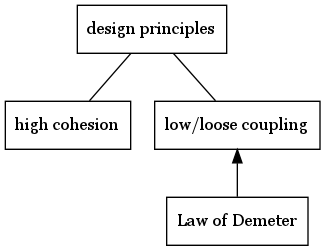
\includegraphics[width=0.5\textwidth]{./graphs/oop_design_principles.png}
  \caption{Znázornění analyzovaných návrhových principů.\label{analyzed_principles}}
\end{figure}

% TODO: v rámci každého návrhového principu uvést příklad porušení
% tohoto principu (případně i příklad, který tento princip dodržuje)

\subsubsection{Low coupling/dependency (nízká závislost/vazba)}
Důležitou návrhovou zásadou je snaha snížit provázanost modulů na minimum. Je možné kategorizovat způsob provázanosti modulů do různých skupin. Následující přehled je převzat z \cite{wiki:coupling} (ještě jemnější dělení je uváděno v \cite{STVR:STVR162}).

\begin{itemize}
\item\emph{Content coupling (nejvyšší forma závislosti)} -- závislost na obsahu modulu -- jeden modul modifikuje nebo se spoléhá na vnitřní fungování jiného modulu (např. přístup k lokálním datům jiného modulu). V důsledku platí, že změní-li se způsob, kterým tento druhý modul produkuje data (umístění, typ, časování), povede to zcela jiste ke změnám v závislém modulu.
\item\emph{Common coupling} -- dva moduly sdílí stejná globální data (např. globální proměnnou), změna sdíleného globálního zdroje implikuje změny všech modulů, které je používají.
\item\emph{External coupling} -- dva moduly sdílí externě definovaný (standardizovaný) datový formát, komunikační protokol nebo rozraní zařízení.
\item\emph{Control coupling} -- jeden modul kontroluje tok druhého tím, že mu posílá informaci o tom, co má konat (např. předání \uv{to-do} příznaku).
  % TODO: CLARIFY
\item\emph{Stamp coupling (Data-structured coupling)} -- mdouly sdílí složenou datovou strukturu a používají pouze její (často odlišnou) část (např. předávání kompletního záznamu funkci, která z něj potřebuje pouze jedno pole). Tato vazba může vést ke změně způsobu, kterým modul čte záznam, protože pole, které tento modul nepotřebuje bylo modifikováno.
  % Stamp coupling is when modules share a composite data structure and use only a part of it, possibly a different part (e.g., passing a whole record to a function that only needs one field of it). This may lead to changing the way a module reads a record because a field that the module doesn't need has been modified.
\item\emph{Data coupling} -- moduly sdílí data pomocí parametrů. Každý parametr je elementární datový typ a jedná se o jediná data, která jsou sdílená (např. předávání celočíselné hodnoty funkci, která spočítá jeho druhou mocninu).
\item\emph{Message coupling (nejnižší forma závislosti)} -- provázanost modulů pouze pomocí zpráv, jedná se o nejnižší úroveň závislosti. Lze jí dosáhnout pomocí decentralizace stavu (u objektů), kde je komunikace dosahováno pomocí parametrů nebo předávání zpráv (\uv{message passing}).
\item\emph{No coupling} -- žádná závislost -- moduly spolu vůbec nekomunikují.
\end{itemize}

%% TODO: sort
%% ## Typy závislostí mezi třídami

%% * třída A dědí ze třídy B
%% * třída A provádí instanciaci třídy B
%% * třída A používá existující intanci třídy B (pracuje s referencí na tuto třídu)

%% Na základě těchto závislostí lze sestavit orientovaný graf. Hrany budeme dále klasifikovat podle toho, o jakou závislost se jedná (dědičnost vs. vyvolání metody).

\subsubsection{High cohesion (vysoká koheze/soudržnost)}
Wikipedia \cite{wiki:cohesion}:
\begin{itemize}
\item míra, jak silně související je funkčnost vyjádřená zdrojovým kódem konkrétního modulu
\end{itemize}

\noindent{}Článek \cite{Kang:1996:DCM:872750.873361}:
\begin{itemize}
\item association-based approach (coincidental, logical, \ldots),
\item slice-based approach,
\item def-use paths,
\item velmi exaktní přístup.
\end{itemize}

\noindent{}Článek \cite{ISI:000079726000029} uvádí dělení koheze podle tzv SMC\footnote{Podle původních autorů Stevens, Myers a Constantine.} Cohesion:
\begin{enumerate}
\item \emph{Coincidental association} -- neexistuje souvislost mezi elementy provádějícími zpracování,
%\item \emph{Coincidental association} -- there is no relationship between the processing elements.
\item \emph{Logical association} -- oba elementy provádějící zpracování patří do stejné logické třídy příbuzných funkcí,
%\item \emph{Logical association} -- both processing elements belong to the same logical class of related functions.
\item \emph{Temporal association} -- každý výskyt obou elementů provadějících zpracování je v tom samém omezeném časovém období při provádění programu,
%\item \emph{Temporal association} -- each occurrence of both processing elements occurs within the same limited period of time during execution.
\item \emph{Procedural association} -- oba elementy provádějící zpracování jsou elementy stejné procedurální jednotky, která je iterativním nebo rozhodovacím procesem,
%\item \emph{Procedural association} -- both processing elements are elements of a common procedural unit which is an iteration or decision process.
\item \emph{Communicational association} -- oba elementy provádějící zpracování pracují nad stejnou množinou vstupních dat a/nebo produkují stejná výstupní data,
%\item \emph{Communicational association} -- both processing elements operate upon the same input data set and/or produce the same output data.
\item \emph{Sequential association} -- výstupní data jednoho elementu jsou vstupními daty pro druhý element,
%\item \emph{Sequential association} -- the output data from one processing element is input to the other processing element.
\item \emph{Functional association} -- oba elementy jsou nezbytné pro provedení jedné funkce/operace.
%\item \emph{Functional association} -- both processing elements are essential to the performance of a single function.
\end{enumerate}

\subsubsection{Law of Demeter}

Existuje několik forem Demeterova zákona \cite{35588}, které jsou vhodné pro různé oblasti aplikace. Tyto typy jsou znázorněny na obrázku \ref{demeter_law_types}. V \cite{35588} se též pojednává o demeterově zákoně z jiného úhlu -- uvažují se všechny možné třídy, které lze volat bez porušení tohto principu (tzv. preferred suppliers).

\begin{figure}[h!]
  \centering
  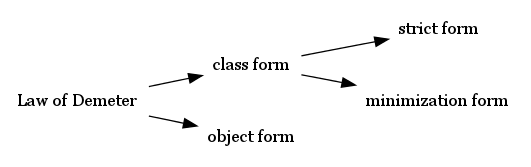
\includegraphics[width=0.7\textwidth]{./graphs/demeter_law_types.png}
  \caption{Formy Demeterova zákona.\label{demeter_law_types}}
\end{figure}

Pro statickou analýzu lze použít \uv{class} formu Demeterova zákona.

TODO: rozhodnout, kterou verzi Demeterova zákona použít

\emph{Zjednodušená verze \cite{wiki:lod}}

Method M of an object O may only invoke the methods of the following kinds of objects:

\begin{itemize}
\item O itself,
\item M's parameters,
\item any objects created instantiated within M,
\item O's direct component objects,
\item a global variable, accessible by O in the scope of M.
\end{itemize}

\subsection{Ukázky kódu porušujících některá z pravidel}

\subsubsection{Porušení principu law of Demeter}

TODO: find some better (real world) example of demeter law violation on the web
\lstset{
    basicstyle=\ttfamily,
    numbers=left,
    numberstyle=\tiny,
    commentstyle=\color{gray}\textit
}
\begin{lstlisting}[language=java]
package violations;

public class DemeterLawViolation {

    void method(MyClass obj, int val) {

        obj.getSomeInternalField().setValue(val);

        // hidden violation:
        InternalFieldDef internalField = obj.getSomeInternalField();
        internalField.setValue(val);

    }

}
\end{lstlisting}

\section{Analýza problematiky v jazyce Java}

\subsection{Statický model programu v Javě}
TODO: pojednání o tom, co všechno může být modelem programu (ast, graf, FSM, programovací jazyky, atd)

TODO: model driven engineering, kód je fyzický model, můžeme jej ale dále převádět na další modely a ty potom analyzovat

TODO: možná přidat poznámku o model driven engineering a jak může být aplikováno právě zde

\subsubsection{Struktura softwarového projektu v Javě}

% TODO: sort and rephrase

\begin{itemize}
\item\verb+*.java+ soubory - v gramatice programovacího jazyka Java 1.5 představují top-level element CompilationUnit \emph{\{(TODO: binární součásti projektu? class files?)\}},
\item build scripty a konfigurační soubory sestavovacích nástrojů (build.xml, pom.xml, \ldots),
\item zdroje (resources),
\item dokumentace,
\item soubory gramatik pro parsery (lex, flex, javacc, \ldots),
\item šablony (typické třeba pro webové projekty),
\item konfigurační soubory (zpravidla XML, často odkazují konkrétní třídy progamovacího jazyka Java),
\item jiné soubory
\end{itemize}

Pro naše potřeby jsou důležité v podstatě pouze kompilační jednotky (java soubory) projektu.

%% TODO: odstranit další výskyty této myšlenky v textu (aby tato věta byla jen na jednom místě)
Statický pohled na program - neuvažujeme běh programu. Pracujeme nad definicemi tříd, nikoliv nad jejich instancemi v paměti JVM.

Projekt závisí na dalších třídách, které analyzovat nebudeme (v určitém okamžiku analýzy je potřeba se \uv{odříznout}, jinak bychom mohli analyzovat všechny knihovny, s nimiž projekt pracuje). Takové závislosti mohou být např.:

\begin{itemize}
\item knihovny třetích stran
\item standardní knihovna jazyka Java (např. Java 2 Platform SE 5.0 API pro Javu verze 5) -- zde například budou povoleny závislosti ze všech modulů (ale pro jiné druhy analýzy to může být nežádoucí - např. u logování budeme chtít, aby v projektu šlo striktně přes nějakou naši konkrétní \emph{fasádu})
\item podprojekty a části projektu, které analyzovat nechceme, nepotřebujeme nebo z nějakého důvodu nemůžeme
\end{itemize}

% TODO: aktualizovat -> v konecnem dusledku budeme pracovat i nad projekty v jazyku 1.6 (protoze nam to rozhrani umoznuje)
Budeme pracovat nad gramatikou jazyka Java 1.5. Java verze 6 se liší pouze úpravou standardních API poskytovaných platformou Java. Jazyk jako takový zůstává stejný.

\subsubsection{Syntaktické elementy programovacího jazyka Java}
Grafické znázornění základních syntaktických elementů, jejichž struktura a názvy jsou převzaty z \cite{Gosling:2005:JLS:1036643}, je na obrázku \ref{toplevel_elements}.
% TODO: write some better accompanying text
\begin{figure}[h!]
  \centering
  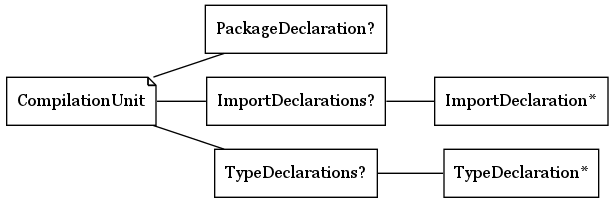
\includegraphics[width=\textwidth]{./graphs/java_top_elements.png}
  \caption{Struktura základních syntaktických elementů programovacího jazyka Java.\label{toplevel_elements}}
\end{figure}

Pro analýzu založenou na vyhledávání závislostí mezi třídami pro nás bude nejdůležitější syntaktický element \emph{TypeDeclaration}. Tento neterminální symbol se dále přepisuje na symboly uvedené na obrázku \ref{type_declaration_options}.

\begin{figure}[h!]
  \centering
  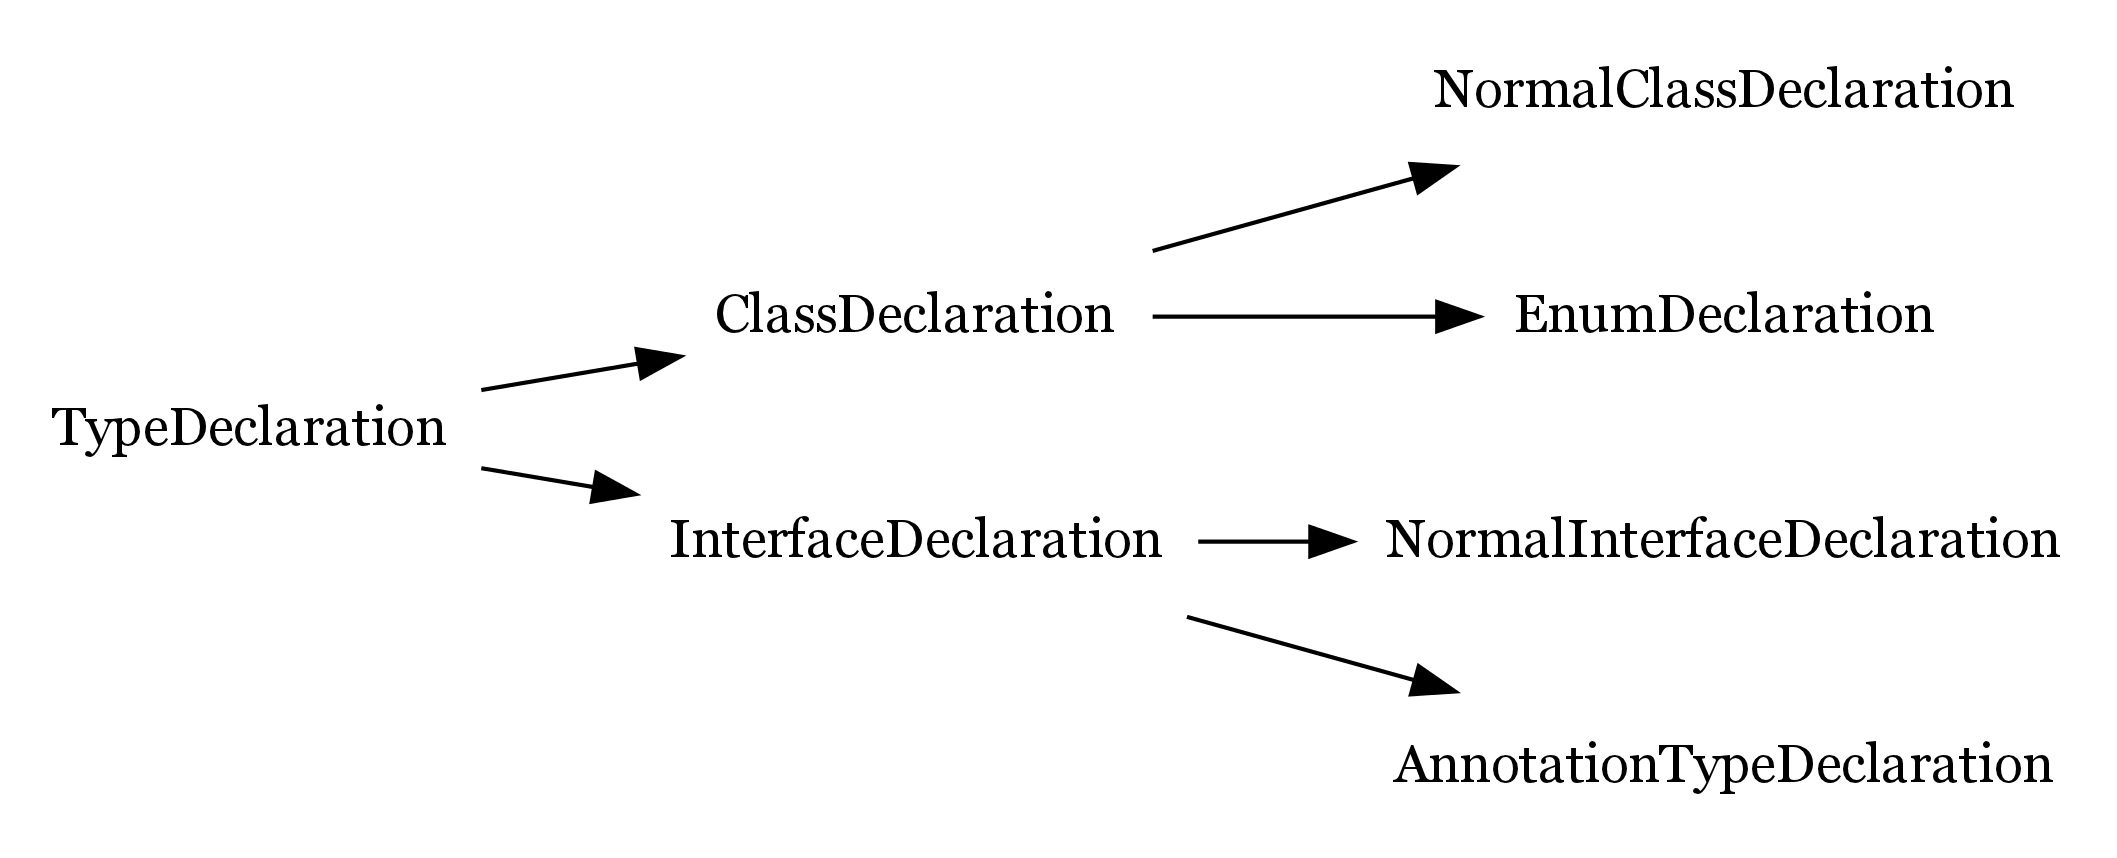
\includegraphics[width=\textwidth]{./graphs/toplevel_types.png}
  \caption{Rozklad elementu TypeDeclaration.\label{type_declaration_options}}
\end{figure}

%% TODO: zatridit tyto syntakticke elementy, ke kazdemu napsat, jak se bude zpracovavat
%% interfaces
%% enums
%% annotations

%% Modifikátory přístupu (private, public, protected, package private) nám umožní "ořezat" graf závislosti tříd.
% Je ale možné, že pro některé druhy analýzy bude toto nežádoucí.

%% ## Speciální případy:

%% * statické třídy
%% * statické metody
%% * vnitřní třídy

%% hlavní analyzované vazby
% instanciace třídy
% dedicnost (inheritance)
% vyvolání metody

%% zpracovávání kódu -> zejména je potřeba resolvovat plná jména a použití elementů v kódu

\subsection{Existující nástroje pro zpracování zdrojových kódů v jazyku Java}

TODO: write some leading text

Možnosti zpracovávání kódu:

TODO: roztřídit a vyházet nesmysly (e.g. JABA, apod.)

TODO: použít jinou vhodnější strukturu místo itemize

\begin{itemize}
\item vlastní hand-written lexikální a syntaktický analyzátor (zbytečně náročné)
\item parser vygenerovaný pomocí některého z dostupných compiler-compiler systémů
  \begin{itemize}
  \item tyto systémy na základě vstupní gramatiky vygenerují frontend pro překladač
  \item lze specifikovat různé akce, které jsou navázány na události vyvolané v průběhu syntaktické analýzy
  \item \emph{JavaCC}
    \begin{itemize}
    \item \href{http://www.cs.purdue.edu/homes/hosking/352/javaccdocs/docindex.html}{http://www.cs.purdue.edu/homes/hosking/352/javaccdocs/docindex.html}
    \item součástí je nástroj \emph{JJTree}, který je schopen vygenerovat AST pro další práci
    \end{itemize}
  \item \emph{JastAdd}
    \begin{itemize}
    \item \href{http://jastadd.org/}{http://jastadd.org/}
    \end{itemize}
  \item \emph{JLex}
    \begin{itemize}
    \item A Lexical Analyzer Generator for Java(TM)
    \item \href{http://www.cs.princeton.edu/~appel/modern/java/JLex/}{http://www.cs.princeton.edu/~appel/modern/java/JLex/}
    \end{itemize}
  \item JFlex
    \begin{itemize}
    \item The Fast Scanner Generator for Java
    \item \href{http://jflex.de/}{http://jflex.de/}
    \end{itemize}
  \item JABA
    \begin{itemize}
    \item \href{http://pleuma.cc.gatech.edu/aristotle/Tools/jaba.html}{http://pleuma.cc.gatech.edu/aristotle/Tools/jaba.html}
    \item Java Architecture for Bytecode Analysis
    \item nepoužitelné - dostupná pouze binární verze pro Solaris
    \item pravděpodobně se dále nevyvíjí
    \end{itemize}
  \end{itemize}
\item použití vhodné knihovny
  \begin{itemize}
  \item JavaParser
    \begin{itemize}
    \item \href{http://code.google.com/p/javaparser/}{http://code.google.com/p/javaparser/}
    \item projekt na GoogleHosting
    \item v podstatě gramatika pro JJTree vytvářející strom tříd a objektů, který je možné procházet pomocí visitor patternu
    \end{itemize}
  \end{itemize}
\item použití prostředků platformy NetBeans
  \begin{itemize}
  \item Retouche API
  \item \href{http://bits.netbeans.org/6.9.1/javadoc/}{http://bits.netbeans.org/6.9.1/javadoc/}
  \end{itemize}
\item použití prostředků poskytovaných platformou Java 6 (Sun verze) \cite{source_code_analysis_corejavatechtips}
  \begin{itemize}
  \item \emph{JSR 199 -- Java Compiler API}
    \begin{itemize}
    \item volání překladače jazyka Java pomocí API ze zdrojového kódu programu
    \item balíček \verb+javax.tools+
    \end{itemize}
  \item \emph{JSR 269 -- Pluggable Annotation Processing API}
    \begin{itemize}
    \item možnost přidání vlastního kódu pro zpracovávání anotací/kódu do instance překladače
    \item balíček \verb+javax.annotation.processing+ -- zpracovávání anotací
    \item balíček \verb+javax.lang.model+ -- třídy poskytující model pro syntaktické elementy jazyka Java
    \end{itemize}
  \item \emph{Compiler Tree API}
    \begin{itemize}
    \item nestandardní rozšíření Java JDK
    \item \href{http://download.oracle.com/javase/6/docs/jdk/api/javac/tree/index.html}{http://download.oracle.com/javase/6/docs/jdk/api/javac/tree/index.html}
    \item balíček \verb+com.sun.source.tree+ -- poskytuje rozhraní pro reprezentaci zdrojového kódu jako AST
    \item balíček \verb+com.sun.source.util+ -- poskytuje rozhraní pro operace nad AST
    \end{itemize}
  \end{itemize}
\end{itemize}

TODO: zatřídit:

Důležité části zpracování kódu:

\begin{itemize}
\item name resolution, jmenné prostory (namespaces), class loaders, class tables
\item static classes, methods
\item inner classes
\item polymorphism
\item vizualizace grafu ?
\item generické třídy, wildcards
\item pole objektů
\item návratové typy metod
\item vstupní parametry metod
\item lokální proměnné
\item globální objekty (statické metody a pole tříd, singletony - opět ale pouze ze statického pohledu!)
\end{itemize}

TODO: zatřídit

úrovně práce:

\begin{itemize}
\item design level -- analýza správného návrhu softwarového díla (pracuje se na konceptuální úrovni, ještě není hotový kód)
\item code level -- analýza existujícího kódu z pohledu návrhu (již máme kód, ale chceme zpětně ověřit, že představuje dobrý/špatný návrh)
\end{itemize}
